\section{Methodology and Our Approach}
\label{sec:our}


\para{Quantum State Discrimination for Localization.} 
Our methodology is to pose the localization problem as a quantum state discrimination problem.
Quantum state discrimination underlies various applications in quantum information processing tasks~\cite{bergou-review-2007}.
It essentially describes the distinguishability of quantum systems in different states, and the general process of extracting classical information from quantum states~\cite{Bae_2015}.
Fig.~\ref{fig:qsd} illustrates the process of quantum state discrimination, where one party (Alice) prepares a quantum state, and another party (Bob) measures the received quantum state sent by Alice.
In our context of localization, the \emph{quantum sensor network plays the role of Alice}.
And a \emph{central node that performs global measurement plays the role of Bob}.
The problem of discriminating among non-orthogonal quantum states boils down to a measurement optimization problem, i.e., optimizing the POVM.
Mathematically, a POVM is a set of positive semi-definite Hermitian matrices $\{E_i\}$ on a Hilbert space $\mathcal{H}$ that sum to the identity matrix, i.e., 
$\sum_{i} E_i = I$.
In quantum mechanics, the POVM element $\{E_i\}$ is associated with the measurement outcome $i$, such that the probability of obtaining it when making a measurement on the quantum state $\rho$ is
\begin{equation}
    Prob(i) = tr(\rho E_i) = tr(\ket{\psi} \bra{\psi} E_i)
\end{equation}
where $tr$ is the trace operator, and $\rho = \ket{\psi} \bra{\psi}$ for pure states.
If we further associate an outcome $i$ with a 2D location $(x, y)$, then we have a location estimator.
For example, we can associate measurement outcomes $i = \{0, 1, 2, 3\}$ to locations $\{(0, 0), (0, 1), (1, 0), (1, 1)\}$ respectively.
So a POVM outputting $1$ indicates the transmitter is at location $(0, 1)$.

\begin{figure}[t]
    \centering
    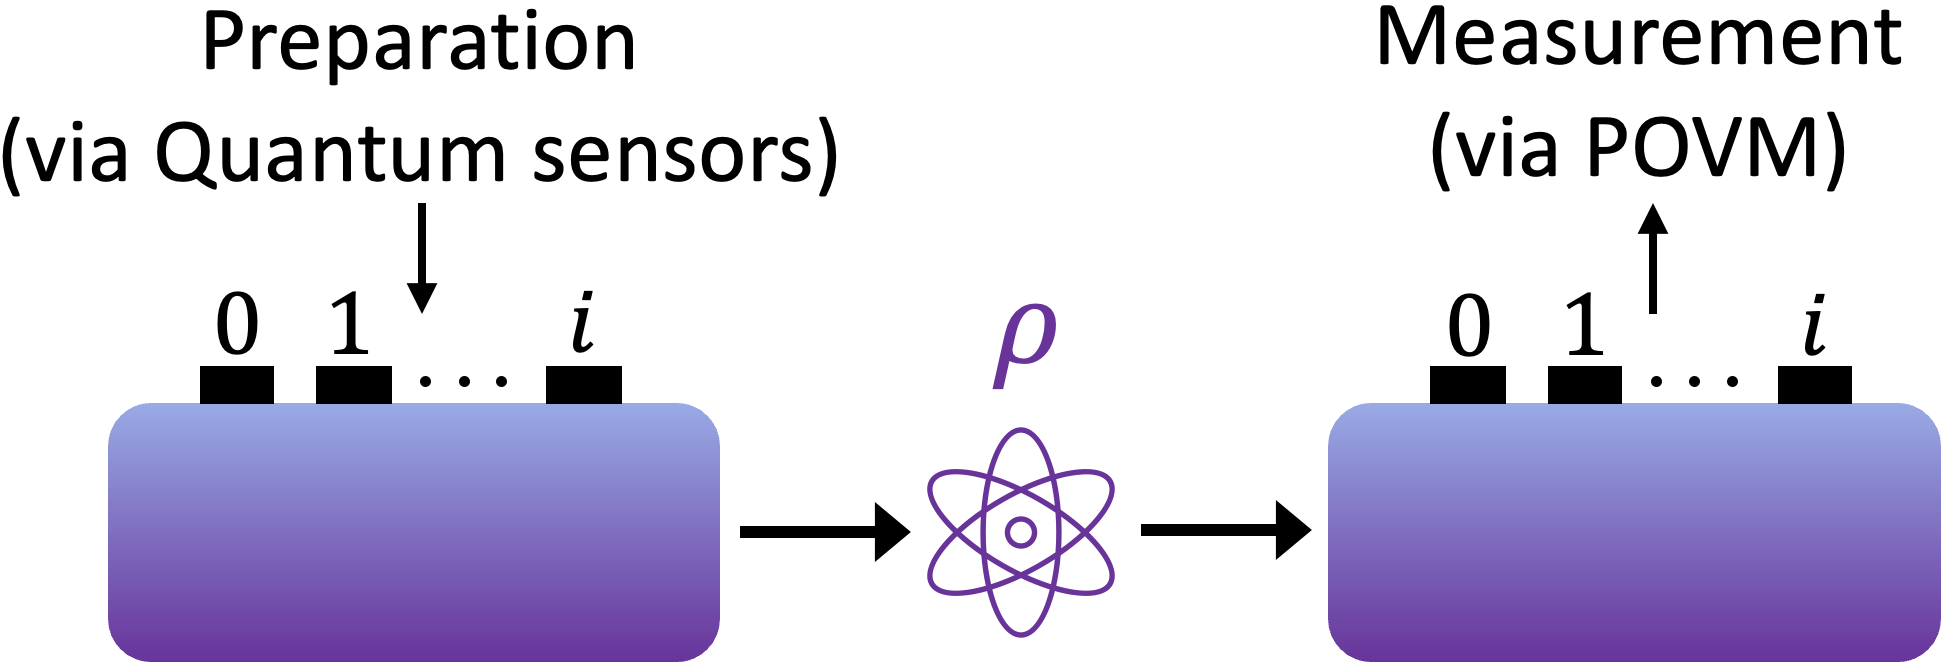
\includegraphics[width=0.5\textwidth]{chapters/icc/figures/qsd.png}
    % \vspace{-0.1in}
    \caption{Illustration of Quantum state discrimination. There are two parties: Alice for preparing and sending a quantum state, and Bob for measuring the received quantum state from Alice.}
    % \vspace{-0.1in}
    \label{fig:qsd}
\end{figure}

Optimizing the POVM is governed by some metrics, such as the minimum error discrimination metric and the unambiguous discrimination metric~\cite{bergou2004}.
Semi-definite programming~\cite{semidefinite} is a general numerical method that can compute the optimal POVM under various metrics.
In our paper, we choose a simple but good enough method to compute a POVM, the pretty good measurement (PGM)~\cite{prettygood}
\begin{equation}
    E_i = p_i \hat{\rho}^{-1/2} \hat{\rho_i} \hat{\rho}^{-1/2}
\end{equation}
where $p_i$ is the prior probability (we assume equal prior for simplicity) for the $i$th quantum state $\hat{\rho_i}$, and $\hat{\rho} = \sum_{i} p_i \hat{\rho_i}$. 
We simulate $\hat{\rho_i}$ through our $\hat{U}(\alpha)$ model as if the transmitter is indeed at the location associated with $i$ and putting the initial probe state $\boldsymbol{\hat{\rho}_0}$ in a uniform superposition state.
\eat{\footnote{Our preliminary results show that an entangled initial probe state (instead of a simple uniform superposition state) will increase the localization performance. But this part is not included due to diluting this paper.}.}

\para{Challenges.}
If we have an appropriate POVM $\{E_i\}$, the localization problem is solved.
But designing the appropriate $\{E_i\}$ has challenges.
1) The first challenge arrives in localization accuracy.
Consider 256 discrete locations in a $16\times16$ grid. 
We can design a POVM that has 256 elements, indicating 256 output locations.
But we observe that a POVM having too many outputs will lead to lower accuracy.
Because when the number of quantum states is high, the difference between each state is relatively smaller (i.e., the overlap between quantum states  is relatively larger). 
Thus being more difficult to discriminate.
So we want to avoid  a POVM that has hundreds of elements.
2) The second challenge is that if we do a global measurement on a relatively high number of sensors, the dimension of the Hilbert space will be large.
It results in POVM elements being too costly in RAM during computation.
Take an example of doing a global measurement on 12 sensors.
Each POVM element will be a complex number matrix of dimension $2^{12} \times 2^{12}$.
Each complex number needs 16 bytes.
A POVM of 256 elements will cost 69 GB of RAM.
In reality, the physical implementation of POVM is costly as well~\cite{pra19-povm}.
So we want to avoid doing a global POVM on tens of sensors.
But if we actually do have tens of quantum sensors, not being able to use all of them is a waste of resources.


\para{Our approach \povm}. A quantum counterpart of the fingerprinting-based approach has a training phase and a localization phase.
\povm is our approach for the localization phase.
The names come from the critical role POVM plays in the approach.
The two challenges mentioned in the previous paragraph can be summarized as the scalability challenge.
In this section, \povm solves the scalability challenge that 1) it has two levels of POVM and each level's POVM needs fewer elements, and 2) utilizes all the given quantum sensors in a novel way that each POVM does a global measurement on fewer number of sensors.
Before describing \povm, we define some concepts.

\begin{itemize}
    \item Grid, block, and cell. We discretize the area into a grid; a cell is the smallest unit in a grid.
    A block is a group of cells. 
    For example, a block in Fig.~\ref{fig:povm-loc} (a) is comprised of $2 \times 2$ cells in  Fig.~\ref{fig:povm-loc} (b).
    
    \item Coarse level and fine level. A coarse level is a level comprised of blocks and a fine level is a level comprised of cells. 
    Fig.~\ref{fig:povm-loc} (a) shows a coarse level with 4 blocks and Fig.~\ref{fig:povm-loc} (b) shows a fine level with 16 cells.
    
    \item Coarse-level sensors and fine-level sensors. A set of coarse-level sensors collects quantum data $ \rho_i $ to determine the block where the transmitter is in. A set of fine-level sensors collects quantum data $ \rho_i$ to determine the cell where the transmitter is in. 
    A set of coarse-level sensors is associated with the grid since it covers the whole grid. A set of fine-level sensors is associated with a block since it only covers a block. 
    Fig.~\ref{fig:povm-loc} (a) has one set of coarse-level sensors, and Fig.~\ref{fig:povm-loc} (b) has four sets of fine-level sensors that cover four blocks (in four colors).
    A sensor at the borders of two blocks covers both blocks.
    
    \item Coarse-level POVM and fine-level POVM. Take $\{ \rho_i \}$ with equal priors and compute the POVM $\{ E_i \}$ using PGM. 
    During the training phase, if $\{ \rho_i \}$ are collected by a set of coarse-level sensors and the transmitter fingerprints at the center of the blocks, we get a coarse-level POVM $\{ cE_i \}$. 
    Likewise, if the  $\{ \rho_i \}$ are collected by a set of fine-level sensors and the transmitter fingerprints at the center of the cell of the associated block, we get fine-level POVM $\{ fE_i \}$.
    Fig.~\ref{fig:povm-loc} (a) shows one coarse-level POVM and Fig.~\ref{fig:povm-loc} (b) shows four fine-level POVMs.
    The dots in Fig.~\ref{fig:povm-loc} indicates the center of a block or cell.
\end{itemize}

\begin{figure}
    \centering
    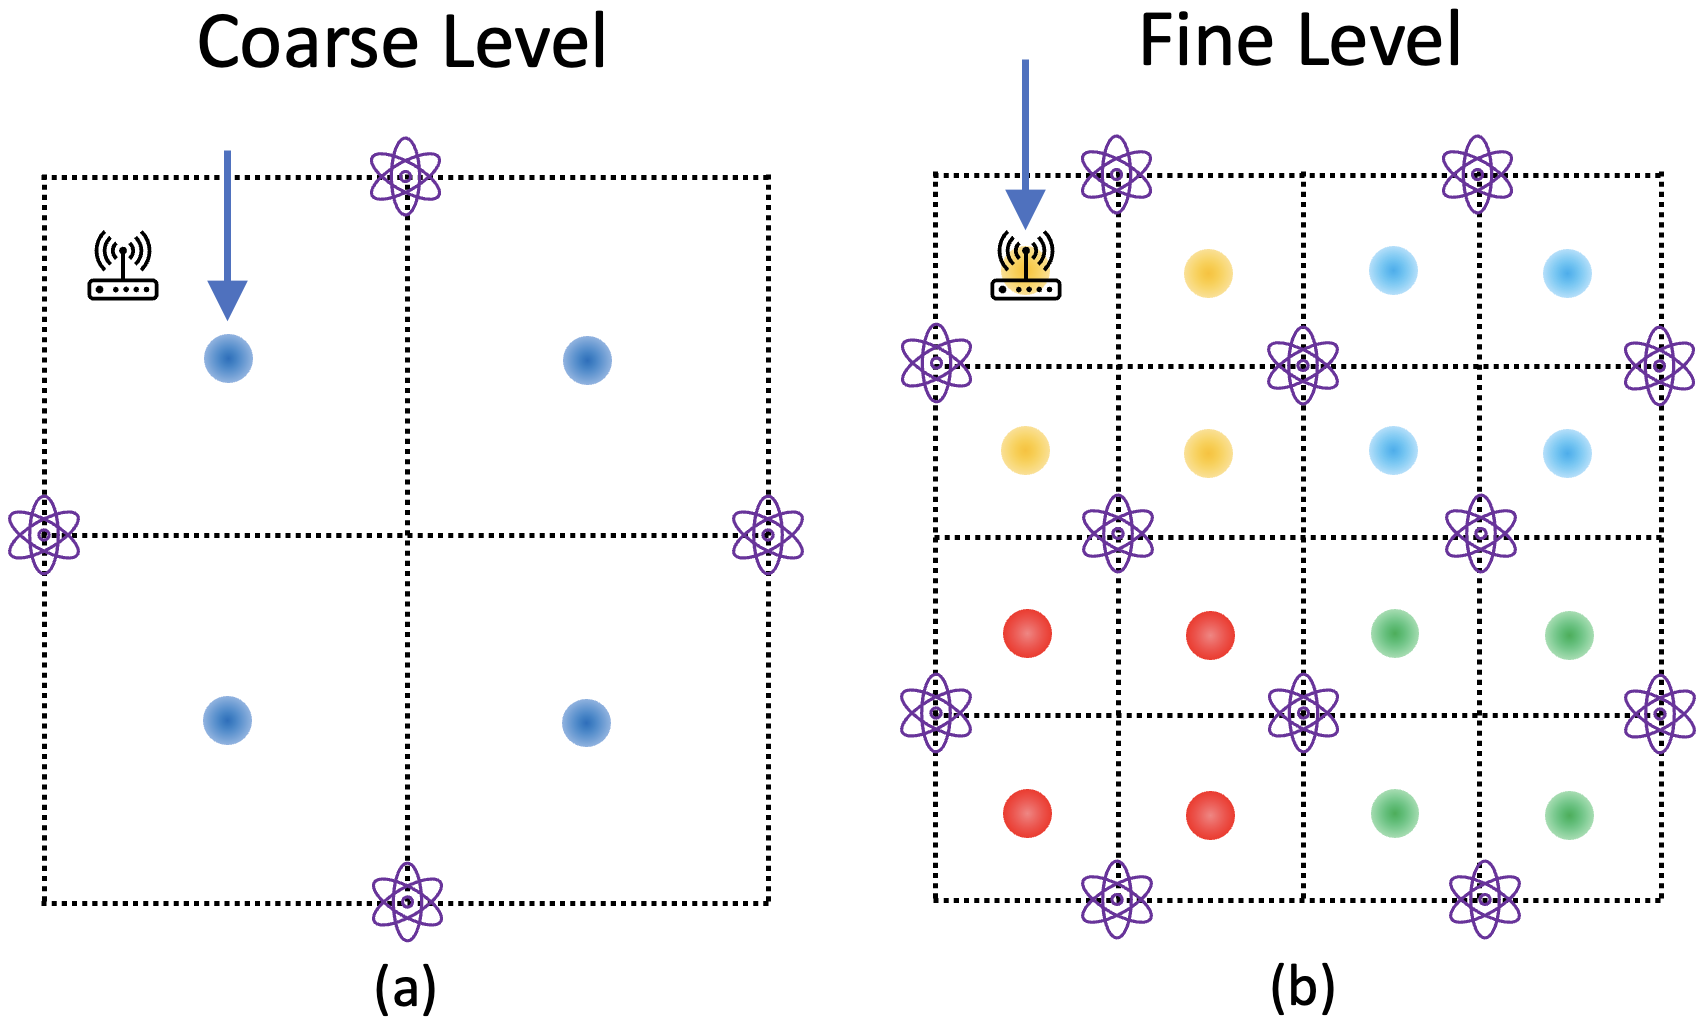
\includegraphics[width=0.6\textwidth]{chapters/icc/figures/povm-loc.png}
    % \vspace{-0.1in}
    \caption{Illustration of \povm, a multi-level POVM scheme for transmitter localization. The coarse level POVM determines the block (a), and the fine level POVM determines the cell (b).}
    % \vspace{-0.1in}
    \label{fig:povm-loc}
\end{figure}

\para{The training phase.}
We discretize an area into a $N\times N$ grid.
Without loss of generality, we assume $\sqrt{N}$ is an integer.
We divide the grid into $\sqrt{N}$ row $\sqrt{N}$ column of blocks whose size is $\sqrt{N}\times\sqrt{N}$.
The sensors will be randomly spread out, ideally close to uniform to better cover the whole area.
For the grid, there will be a set of coarse-level sensors associated with the grid, and the coarse-level POVM is computed by quantum data collected from the coarse-level sensors.
For each block, there will be a small number of sensors associated with the block. 
Each block's fine-level POVM is computed by quantum data collected from the block's associated fine-level sensors.


\begin{algorithm}[ht] 
  	\KwIn{$\{cE_i\}$ -- one coarse-level POVM}
        \KwIn{[$\{fE_i^{0}\}, \{fE_i^{1}\}, \cdots$] -- an array of fine-level POVMs}
	\KwOut{location $(x, y)$}
        $repeat \leftarrow$ 1000 \;	
        $j \leftarrow$ SenseMeasure($\{cE_i\}$, $repeat$) \;
        $block_j \leftarrow$ the block associated with $j$ \;
        $\{ fE_i\} \leftarrow$ the fine-level POVM associated with $block_j$ \;
        $j \leftarrow$ SenseMeasure($\{fE_i\}$, $repeat$) \;
        $cell_j \leftarrow$ the cell associated with $j$ \;
        % \uIf{$cell_j$ is at the edge of two blocks}{
        %     $block_e \leftarrow$ the block that covers the edge of the two blocks \;
        %     $\{ fE_i\} \leftarrow$ fine-level POVM associated with $block_e$ \;
        %     $j \leftarrow$ SenseMeasure($\{fE_i\}$, $repeat$) \;
        %     $cell_j \leftarrow$ the cell associated with $j$ \;
        % }
        \Return the location $(x, y)$ of $cell_j$ \;
	\caption{\povm}
\label{algo:povm-loc}
\end{algorithm}
% \vspace{-0.25in}
\begin{procedure}[ht]
    \KwIn{$\{E_i\}$ -- a POVM}
    \KwIn{$K$ -- number of repetition}
    \KwOut{$j$ -- the most frequent measurement outcome}
    $count \leftarrow$ a key-value pair dictionary\;
    $qsensors \leftarrow$ a set of quantum sensors associated with the POVM $\{E_i\}$ \;
    \For{$k=1 \cdots K$}{
        $\rho \leftarrow $ a quantum state sensed by $qsensors$ \;
        $i \leftarrow$ outcome of measuring $\rho$ via POVM $\{E_i\}$ \;
        $count[i] =  count[i] + 1$ \;
    }
    $j \leftarrow arg\,max_{\{ i\}} \ count[i]$ \;
    \Return $j$ \;
    \caption{SenseMeasure($\{E_i\}$, $K$)}
\label{algo:sense-measure}
\end{procedure}
% \vspace{-0.1in}
\para{The localization phase.}
At a higher level, \povm localizes a transmitter from a coarser level to a finer level.
Without any prior information, a transmitter could be anywhere in the area.
The coarse-level POVM's output can decrease the scope of the area from the whole grid to a block.
Then inside a block, a fine-level POVM's output will determine where the cell the transmitter is in.
Algorithm~\ref{algo:povm-loc} is the pseudo-code of \povm.
Algorithm~\ref{algo:povm-loc} relies on Procedure~\ref{algo:sense-measure} that repeats the process of state preparation via a quantum sensor network and POVM measurement and returns the most frequent measurement output. 
Procedure~\ref{algo:sense-measure} can be viewed as the quantum sensing protocol~\cite{RevModPhys.quantumsensing} in our localization context.


\para{A further improvement \povmpro.} Through the two-level scheme, \povm avoids doing a global measurement on a large number of quantum sensors and having a large number of elements in a POVM, thus being scalable. 
Through evaluation, the scheme works quite well. However, we observe that the cells at the edge of the blocks have a higher chance of error in localization.
Another observation is that the wrong output cell of \povm is usually nearby to the correct cell, like the other side of the border.
To mitigate this kind of error, we put a new block that covers the border of the blocks.
These new blocks are called border blocks and each border block will be associated with a set of fine-level sensors (previous fine-level sensors can be reused).
So, whenever \povm returns a cell at the border of blocks, we find the border block where the cell is inside and do a second fine-level POVM associated with the border block.
Then the outcome of the second fine-level POVM is the final return.
This scheme of \povm plus an optional second fine-level POVM is named \povmpro.
See Fig.~\ref{fig:povmloc-pro}.


\begin{figure}[t]
    \centering
    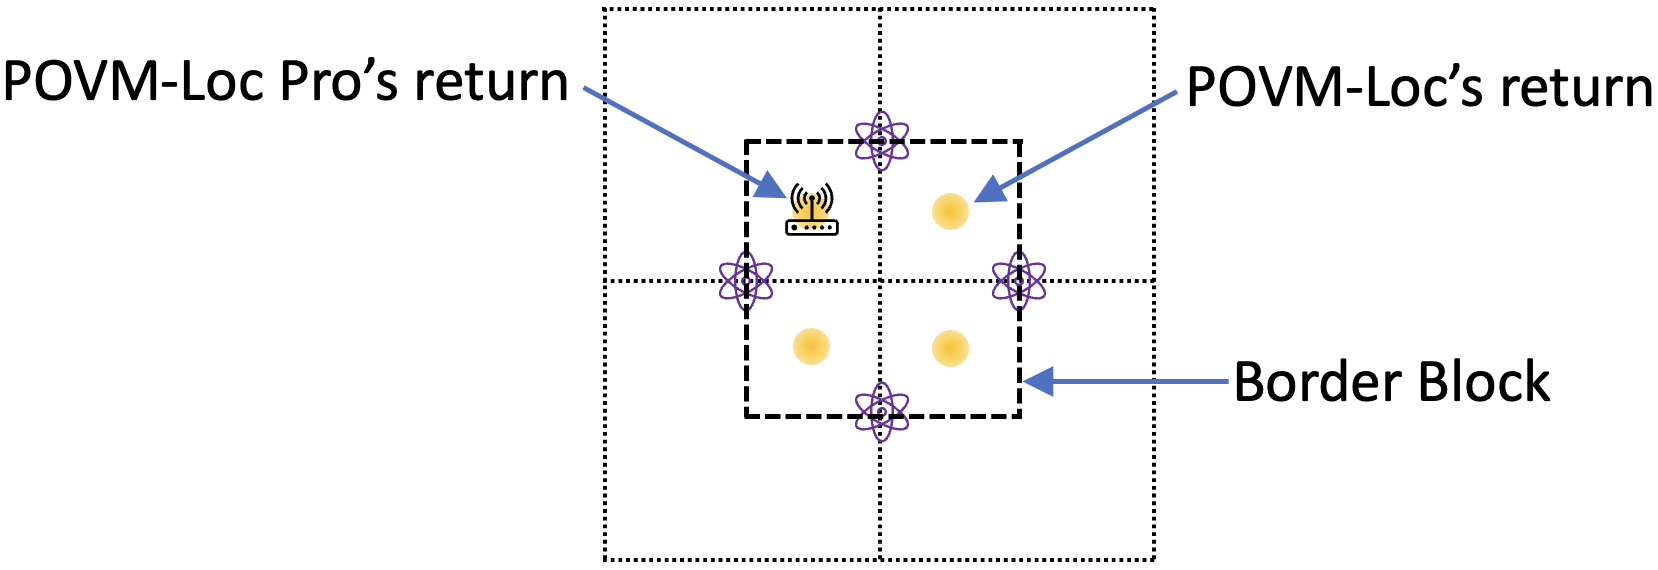
\includegraphics[width=0.8\textwidth]{chapters/icc/figures/povm-loc-pro.png}
    % \vspace{-0.1in}
    \caption{Illustration the idea of \povmpro. There are four blocks and one border block in the middle. 
    If \povm returns a cell that is at the edge of a block, do another fine-level POVM associated with the border block.}
    % \vspace{-0.1in}
    \label{fig:povmloc-pro}
\end{figure}


